% Suppress some compilation warnings
\RequirePackage[save,showerrors]{silence}
\WarningFilter{biblatex}
  {The starred command '\DeclareDelimAlias*' is} % APA package is using this deprecated starred version
\WarningFilter{transparent}
  {Loading aborted} % I can't find where it is loaded, probably somewhere in kao's cls or sty
\WarningFilter{latex}
  {Unused global option} % They are, but kaobook is silently passing them to its base class
\WarningFilter{latex}
  {Marginpar on page} % Margin stuff moved to not overlap with other stuff, this is fine
\WarningFilter{latex}
  {There were undefined references} % seems spurious, no undefined references are reported
\WarningFilter{biblatex}
  {Please (re)run Biber on the file} % linked to the previous warning

\documentclass[
    a4paper,
    chapterentrydots=true,
    fontsize=11pt,
    open=any,      % Force new chapters to start on any page, not only on right (odd) pages
    secnumdepth=1, % How deep to number headings (1 = sections)
    twoside=true,  % Use different layouts for even and odd pages
]{kaobook}

% TODO: show the page number on each page (unless forbidden by the dissertation requirements)

% Code highlighting
\usepackage{minted}

% Main and default language is french but there are some parts in english
\usepackage[main=french,english]{babel}
\newcommand{\en}[1]{\foreignlanguage{english}{\itshape #1}}
\usepackage{csquotes}
\MakeOuterQuote{"}

% Allow to include SVG with \includesvg similarly to \includegraphics for other image formats
\usepackage[inkscapepath=./build/svg-inkscape/]{svg}

% Bibliography configuration
\usepackage[style=apa]{kaobiblio}
\DefineBibliographyExtras{french}{\restorecommand\mkbibnamefamily}
\addbibresource{references.bib}
% Properly cite articles indirectly cited via meta-analysis, this mimics the \nocitemeta command from apacite
\DeclareBibliographyCategory{meta}
\renewbibmacro*{begentry}{\ifcategory{meta}{\ensuremath{{}^\ast}}{}}
\newcommand*{\nocitemeta}[1]{\nocite{#1}\addtocategory{meta}{#1}}

% Hyperref integration
\usepackage{kaorefs}
\usepackage[nobiblatex]{xurl}

% For typesetting hypothesis
\usepackage[framed=true, hypothesisbackground=gray!20!white]{kaotheorems}
\usepackage{thmtools}
\usepackage{thm-restate}

% For file inclusion and figure formatting
\usepackage{svg} % for svg images
\usepackage{caption}
\captionsetup[subfigure]{justification=centering}
\usepackage{subcaption}
\usepackage{pdfpages}

% Search paths for images and tex input files
\graphicspath{{images/}}

% Configure the index and the glossary
\makeindex[columns=3, title=Alphabetical Index, intoc]
\makeglossaries
\setglossarystyle{altlist} % TODO: switch to altlistgroup if I end up with a lot entries
% Accronyms
\newacronym{gpl}{GPL}{GNU General Public License}
\newacronym{cc}{CC}{Creative Commons}
\newacronym{OSL}{OSL}{Open Source Lab}

% Glossary
\newglossaryentry{commit}{
    name=\en{commit},
    description={
        Une contribution au code. Un \en{commit} est l'enregistrement d'un petit ensemble de modifications
        (suppression, ajout ou modification de une ou plusieurs lignes, dans un ou plusieurs fichiers) apporté
        au code source d'un projet
    },
}

\newglossaryentry{git}{
    name=git,
    description={
        \url{https://git-scm.com/}\\
        Un système de versionnement. Git est un logiciel permettant de sauvegarder l'historique de
        développement d'un projet (ses \englpl{commit}) et d'organiser les contributions d'un petit ou grand
        nombre de personnes. Il est pensé pour mais pas limité aux logiciels libre, git a été conçu à
        l'origine pour organiser le développement du noyeau de système d'exploitation \gls{linux}).
        L'historique d'un projet tel que sauvegardé par Git est communément appelé un "\gls{dépôt} Git"
    },
}

\newglossaryentry{dépôt}{
    name=dépôt,
    description={Voir \gls{git}},
}

\newglossaryentry{linux}{
    name=Linux,
    description={\url{https://www.kernel.org/}\\Un système d'exploitation libre},
}

\newglossaryentry{github}{
    name=GitHub,
    description={
        \url{https://github.com/}\\
        Une plateforme d'hébergement de \glspl{dépôt} \gls{git}, gérée par une entreprise privée
    },
}

\newglossaryentry{gitlab}{
    name=GitLab,
    description={
        \url{https://about.gitlab.com/}\\
        Un logiciel libre permettant de créer des plateformes d'hébergement de \glspl{dépôt} \gls{git}
    },
}

\newglossaryentry{fosdem}{
    name=FOSDEM,
    description={
        \url{https://fosdem.org}\\
        Acronyme de "\en{Free and Open Source Developers' European Meeting}". Il s'agit d'une conférence
        annuelle à l'accès gratuit hébergeant le temps d'un week-end de nombreuses présentations, ateliers et
        discussions autour du logiciel libre
    },
}

\newglossaryentry{synva}{
    name=SYNVA,
    description={
        \href{https://sfc.unistra.fr/formations/formation_-_ingenierie-de-formation_-_master-2-ingenierie-des-systemes-numeriques-virtuels-pour-lapprentissage-synva_-_2393/}
             {\nolinkurl{https://sfc.unistra.fr/[...]}}\\
        Master 2 ingénierie des SYstème Numériques Virtuels pour l'Apprentissage. Une formation dispensée par
        l'université de Strasbourg
    },
}

\newglossaryentry{epita}{
    name=EPITA,
    description={
        \url{https://www.epita.fr/}\\
        École d'ingénieurs privée, acronyme de "École pour l'Informatique et les Techniques Avancées"
    },
}

% shortcut for english glossary entries
\newcommand{\engl}[1]{\en{\gls{#1}}}
\newcommand{\enGl}[1]{\en{\Gls{#1}}}
\newcommand{\englpl}[1]{\en{\glspl{#1}}}
\newcommand{\enGlpl}[1]{\en{\Glspl{#1}}}

% Deactivate the citation/figure margin for new part pages
\NewCommandCopy{\oldaddpart}{\addpart}
\renewcommand{\addpart}[1]{%
    \pagelayout{wide} % no citation/figure margin
    \oldaddpart{#1}
    \pagelayout{margin} % restore the margin
}

% Hyphenation
\hyphenation{Git-Hub}

\begin{document}
    % Book information
\titlehead{}
\title{L'identification des projets de logiciel libre accessibles aux nouveaux contributeurs}
\subtitle{Mémoire de Master Sciences de l'Éducation, parcours SYNVA}
\author[PH]{Soutenu par\\Paul HERVOT}
\date{le 8 septembre 2022}
\publishers{
    Mémoire présenté en vue de l'obtention du Grade de Master

    \bigskip
    \bigskip
    \bigskip
    \bigskip

    Commission de soutenance composée par :

    \bigskip

    \begin{tabular}{lr}
        Benoît CRESPIN & directeur\\
        Richard NGU LEUBOU & assesseur
    \end{tabular}

    \bigskip

    \begin{figure}[ht]
        
\includegraphics[width=0.45\textwidth]{inspe_unistra}
        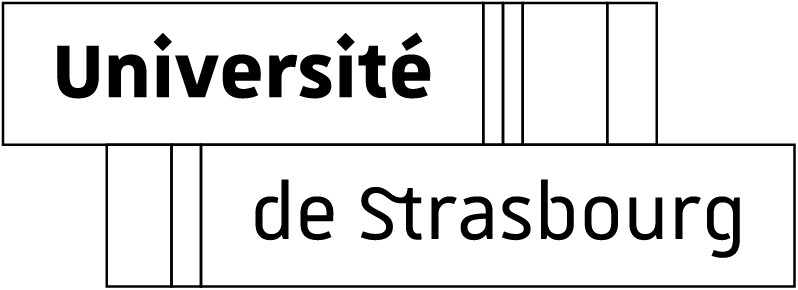
\includegraphics[width=0.45\textwidth]{unistra}
    \end{figure}
}
\dedication{%
    Un grand merci à Antoine Pietri pour son aide précieuse lors de la collecte des données sur le graphe de
    Software Heritage.

    \emph{Deux} grands mercis à Marc Trestini et Benoît Crespin, ayant par la force des choses tous deux
    endossé le rôle de directeur de ce mémoire à différentes étapes de son écriture, leurs expertises
    complémentaires m'a permis d'arriver au bout de ce travail si nouveau pour moi.%
}

% Pre-document content
\setchapterstyle{plain}
\pagelayout{wide}

% Copyright page
\makeatletter
\uppertitleback{\@titlehead}
\lowertitleback{
    \textbf{Pas de copyright} \\
    \ccby\ Ce mémoire est mis à disposition selon les termes de la
    \href{https://creativecommons.org/licenses/by/3.0/fr/}{Licence Creative
    Commons Attribution}.

    \medskip

    \textbf{Colophon} \\
    Ce document a été composé avec l'aide de
    \href{https://sourceforge.net/projects/koma-script/}{\KOMAScript} et
    \href{https://www.latex-project.org/}{\LaTeX} en utilisant la classe
    \href{https://github.com/fmarotta/kaobook/}{kaobook}.

    \medskip

    \textbf{Éditeur} \\
    Première publication le TODO par l'Université de Strasbourg % TODO date
}
\makeatother

% Note that \maketitle outputs the pages before here
\maketitle

\chapter*{Préface}

% Table of contents, figures and tables
\begingroup % Local scope for the following commands
    \tableofcontents

    \listoffigures

    % Keep the list of figures and the list of tables on the same page
    \let\cleardoublepage\bigskip
    \let\clearpage\bigskip

    \listoftables
\endgroup


% Main document content
\pagestyle{scrheadings}
\setchapterstyle{kao}

\pagelayout{margin}
\chapter{Introduction}

\section{Le logiciel libre}

Au cours des quelques décennies précédentes, le numérique s'est développé pour intégrer et assister la plupart
des domaines de recherche, des secteurs industriels, ainsi que des aspects de nos vies. Son champ est
aujourd'hui très vaste et connaît en son sein de nombreuses dynamiques différentes ayant un impact sur ses
domaines d'applications, parmi lesquelles celle du logiciel libre.

En essence, les logiciels, applications, services numériques et autres programmes sont des ensembles
d'instructions compréhensibles par un ordinateur et lui indiquant comment utiliser ses ressources afin de
réaliser un certain nombre de tâches. Pour être utilisables par un ordinateur, ces instructions doivent être
formulées en "code machine", un langage souvent représenté en binaire et extrêmement difficile à manipuler par
les humains, même les plus spécialisés, aussi bien en ce qui concerne son écriture que sa compréhension. C'est
pourquoi lors de la création d'un logiciel, les développeurs décrivent d'abord le comportement souhaité dans
un autre langage, textuel et raisonnablement maîtrisable pour un être humain spécialisé, que l'on appelle un
"langage de programmation". Cette description textuelle du logiciel est ce que l'on appelle son "code source",
il est ensuite traduit en code machine par un autre programme (généralement appelé un "compilateur") avant
d'être livré aux personnes souhaitant utiliser le logiciel.

Pour utiliser un logiciel, nous n'avons donc besoin que de son code machine, mais c'est seulement en lisant
son code \emph{source} que l'on peut vraisemblablement comprendre son fonctionnement, corriger ses éventuelles
erreurs, l'adapter à d'autres besoins, vérifier la présence de comportements malveillants, etc. La question de
rendre publiquement disponible le code source d'un logiciel est un enjeu faisant souvent intervenir plusieurs
intérêts divergents, allant de la transparence du fonctionnement de certains services et leur gestion
démocratique au secret industriel.

L'expression "logiciel libre" désigne en français un logiciel disponible publiquement et gratuitement dont le
code source est lui aussi disponible publiquement et gratuitement, ainsi que sa modification et sa
redistribution par toutes et tous. Cette expression désigne aussi et surtout un mouvement visant à développer
la part de logiciel libre dans le numérique, un mouvement dans lequel se développe toute une culture, des
pratiques, des fondations et des événements internationaux. L'expression équivalente anglaise, "\en{Free and
Open Source Software}" (FOSS) est souvent utilisée dans les références citées dans ce mémoire.

\section{Mon parcours personnel}

Étant issu d'une formation d'ingénieur spécialisée en informatique, mon domaine d'expertise se situe
principalement dans le numérique, et en particulier dans le développement logiciel. Mon parcours m'a
rapidement amené au logiciel libre, notamment via les technologies utilisées au sein de mon école d'ingénieur,
l'\gls{epita}, mais surtout via mon implication pendant mes études dans des associations comme
Prologin\sidenote{\url{https://prologin.org}} et GConfs\sidenote{\url{https://gconfs.fr}} : l'une organisant
un concours francophone d'algorithmique ainsi que des stages d'initiation à l'informatique pour
lycéennes\sidenote{\url{https://girlscancode.fr/}}, l'autre œuvrant au partage de connaissance entre pairs en
organisant des conférences par les élèves et pour les élèves au sein de l'école. Ces deux associations ont
produit des sites web ainsi que de nombreux outils informatiques, tous sur le principe du logiciel libre, ce
qui a beaucoup contribué aux échanges avec leurs publiques cibles en permettant à tous de participer,
commenter et améliorer les outils développés, en plus d'accroitre la transparence de leurs structures.
Plusieurs des outils développés par ces associations ont d'ailleurs été réutilisés dans d'autres contextes par
d'autres personnes qui leurs sont externes. Cette implication dans le mouvement du logiciel libre m'a aussi
amené à assister régulièrement au \gls{fosdem}\sidenote{\url{https://fosdem.org}}, la conférence principale du
logiciel libre en Europe, aussi bien l'occasion de s'informer sur l'évolution des nombreuses communautés du
logiciel libre qu'un prétexte pour y retrouver de vieilles connaissances lors d'un week-end à Bruxelles.

Mon parcours s'est ensuite enrichi d'une expérience dans l'enseignement lorsque j'ai rejoint pendant ma
cinquième et dernière année à l'\gls{epita} la petite équipe des "assistants", qui encadre l'enseignement de
la principale matière informatique pour les étudiants de troisième année. J'ai écrit et évalué au sein de
cette équipe des sujets de travaux pratique et encadré de nombreuses séances de travail sur ordinateur, ce qui
a développé chez moi une forte appétence pour l'enseignement. J'ai souhaité explorer cette appétence après la
fin de mes études lors d'un service civique au collège et lycée Jean Monnet de Strasbourg, où j'y ai donné des
cours de soutient. Ayant confirmé mon intérêt pour cette voie professionnelle, je suis revenu à l'\gls{epita}
pour y devenir enseignant des matières informatiques, à l'occasion de l'ouverture de son nouveau campus à
Strasbourg.

Enfin, de nombreuses discussions avec des amis chercheurs et passionnés de méthodologie scientifique, ainsi
qu'une tentative personnelle pour me familiariser avec la recherche en éducation, m'ont poussé à entreprendre
une formation m'aidant d'une part à développer mes connaissances en éducation, et me fournissant d'autre part
une introduction à la recherche scientifique, tout en exploitant mes acquis en informatique. C'est ainsi que
je me suis inscrit au Master SYNVA et que je cherche, à travers ce mémoire, à explorer et contribuer à la
recherche touchant ces domaines de l'informatique, de l'enseignement, ainsi que de la libération de la
connaissance et de l'information.

\section{Les projets de logiciel libre dans l'enseignement de l'informatique}

La pédagogie de projet est une méthode d'enseignement qui consiste à inviter les apprenants à appliquer leurs
connaissances et à en acquérir de nouvelles au travers d'un projet plus ou moins concret et imitant plus ou
moins fidèlement une situation réelle. Réalisé soit individuellement soit en groupe, les projets aboutissent
généralement à une production évaluée par l'enseignant, parfois au travers d'une présentation donnée par les
apprenants. L'efficacité de cette méthode a fait l'objet de nombreuses recherches au cours des années
précédentes. Plusieurs méta-analyses concluent que cette méthode a des effets mesurables, positifs et
importants sur les résultats académiques des apprenants en sciences sociales et en sciences naturelles
\sideparencite{pbl-2019, pbl-2018}.

Les projets proposés aux étudiants sont le plus souvent factices, imaginés par les enseignants dans le seul
but de servir d'exercice. Utiliser au contraire des projets réels, qui ne cessent pas d'exister après la fin
de la séquence pédagogique, sur lesquels faire travailler les étudiants donne des résultats encore meilleurs,
mais est aussi plus difficile et incertain à encadrer pour les enseignants \sideparencite{real-pbl-2010,
real-pbl-2004}. Il est notamment très difficile pour l'enseignant de prévoir à l'avance les problèmes que les
apprenants risquent de rencontrer, c'est pourquoi d'autres efforts dans cette direction ont tenté un
compromis, consistant à créer des projets de logiciel libre aussi proches des situations réelles que possible,
mais dédiés à l'éducation \sideparencite{oss-edu-2008}. Les projets en question ne sont cependant plus
accessibles aujourd'hui, une explication possible à leur disparition étant leur portée réduite à l'éducation
et l'absence d'une communauté persistante autour d'eux.

Bien qu'elles soient plutôt rares, quelques initiatives existent aussi pour enseigner spécifiquement les
pratiques du logiciel libre dans l'éducation supérieur et la formation tout au long de la vie. Certaines sont
des initiatives venant des communautés du logiciel libre, comme le \en{Professional Certificate in Open Source
Software Development, Linux and Git}%
\sidenote{\url{https://www.edx.org/professional-certificate/linuxfoundationx-open-source-software-development-linux-and-git}}
de la \en{Linux Foundation}, et en particulier la première séquence : \en{Open Source Software Development:
Linux for Developers}%
\sidenote{\url{https://www.edx.org/course/open-source-software-development-linux-for-developers}} ; ou les
séminaires de l'\en{open source initiative}\sidenote{\url{https://opensource.org/osi-open-source-education}}.
Enfin, certaines universités proposent des cursus en informatique ayant des éléments visant spécifiquement les
pratiques du logiciel libre, c'est le cas notamment de l'Université de l'État de Caroline du Nord aux
États-Unis, qui a expérimenté plusieurs façons d'inclure la contribution aux projets de logiciel libre dans
leurs cursus d'informatique \sideparencite{oss-edu-2008, oss-edu-2007} ; mais aussi de l'université de Calais
qui propose actuellement un "Master Informatique - Ingénierie du logiciel libre"%
\sidenote{\url{https://www.univ-littoral.fr/formation/offre-de-formation/masters/master-informatique-ingenierie-du-logiciel-libre/}},
sous la forme d'une formation en alternance.

\pagelayout{wide}

\addpart{Partie théorique}

\pagelayout{margin}
\chapter{Revue de littérature}

\section{TODO article lus mais sans catégorie}

\sidetextcite{strategies-2012} identifient cinq grandes étapes dans les interactions que les entreprises ont
généralement avec les logiciels libres :
\begin{description}
    \item[identification] -- évaluer la qualité d'un logiciel libre, ses garanties et les potentiels brevets
        utilisés ;
    \item[adoption] -- utilisation du logiciel ;
    \item[conformité] -- examen des licence attachées au logiciel, de leur compatibilité avec les activités de
        l'entreprise, et des contraintes qu'elles apportent dans les activités futures ;
    \item[contribution] -- partage avec la communauté.
\end{description}

\textcite{strategies-2012} notent un grand besoin de formation au sein des entreprises sur le sujet des
licences, ainsi qu'un intérêt pour celle-ci à participer aux projets qu'elles utilisent.

Au sein d'un projet de logiciel libre, la communauté produit généralement plus de \englpl{commit} que de
messages sur les listes de diffusion, mais il y a une corrélation entre le nombre de \englpl{commit} et le
nombre de messages que chaque développeur écrit \sideparencite{contribution-patterns-2010}. Cela indique qu'au
sein d'un projet de logiciel libre, bien que la production de \englpl{commit} prend plus de place, les
contributeurs participent aux échanges sur les listes de diffusion proportionnellement au nombre de
\englpl{commit} qu'ils font. Si l'on souhaite enseigner ces comportements aux étudiants, il ne faut donc pas
négliger cet aspect communication.

\section{Les barrières d'entrée}

\sidetextcite{barriers-2018} notent la difficulté des nouveaux volontaires à rejoindre une communauté de
logiciel libre, citant comme exemple extrême le projet \en{Apache Hadoop} voyant 82\% de ses nouveaux
volontaires quitter le projet après leur première contribution \sideparencite{hadoop-dropout-2013} (TODO: lire
cet article en détail et comprendre les nuances). Les études, que \textcite[p.~1005]{barriers-2018} citent,
mentionnent deux approches différentes de la résolution de problèmes observées dans les projets informatique :
l'une consiste à d'abord rassembler le plus d'informations possibles sur le problème avant de tenter en un
deuxième temps de le résoudre (approche statistiquement plus commune chez les femmes que les hommes), l'autre
consiste à agir sur la première information ou piste prometteuse trouvée, quitte à revenir en arrière et
chercher de nouvelles informations si elles n'étaient pas concluantes (approche statistiquement plus commune
chez les hommes que les femmes). De façon peut être plus importante pour ce mémoire, et toujours d'après les
études citées par \textcite[p.~1005]{barriers-2018}, on observe deux façons d'apprendre les fonctionnalités
d'un logiciel statistiquement préférées de façon inégales selon le genre : l'une, statistiquement plus
probable chez les femmes, consiste à les apprendre méthodiquement en suivant des processus d'apprentissage
clairs. L'autre, statistiquement plus probable chez les hommes, consiste à expérimenter à la manière d'un jeu
avec ces fonctionnalités. TODO : je dis beaucoup "les études citées par <truc>", il faudrait modifier ça pour
citer les vrais auteurs des informations dont je parle. Une des tendances trouvées par
\textcite[p.~1008]{barriers-2018} est que la majorité ($58\%$) des barrières rencontrées dans leur étude sont
de nature sociale ("\en{community-oriented}") et non techniques. Concernant les aspects plus techniques, il
semble que les outils et la documentation représentent la majorité des barrières rencontrées, alors même que
ces éléments ont spécifiquement pour objectif d'aider les nouvelles contributions. C'est un type de barrière
qui semble amplifié lorsque les méthodes d'apprentissage et de traitement de l'information de la personne
consistent à rassembler le plus d'information possible avant de commencer à agir. Ces méthodes étant
sur-représentées chez les femmes, ces barrières devient discriminantes selon le genre, et peuvent
potentiellement participer à expliquer la sous-représentation des femmes dans les communautés de logiciel
libre. \textbf{TODO : je me suis cette fois arrêté avant la partie 4 "\en{RELATED WORK}", page 1010}.

Il a été théorisé et souvent observé de façon générale que la diversité de genre, d'origines et d'ancienneté
au sein d'une équipe augmente sa productivité (TODO : trouver une citation générique). C'est ce que
\sidetextcite{diversity-2015} ont pu confirmer dans le cas précis des projets de logiciel libre hébergés sur
\gls{github}. Ils mettent cette observation en persective avec celle de la proportion de
femmes dans ce type d'équipe, en très forte minoritée, et concluent en suggérant que des efforts
supplémentaires d'inclusivité et de réduction des barrières d'entrée pour ces population en minorité
permettraient probablement d'augmenter la valeur globale de ce type de projets.

Liste de barrières d'entrée que rencontrent les nouveaux arrivants dans un projet de logiciel libre :

\begin{itemize}
    \item l'identification d'une tâche par laquelle commencer \sideparencite{first-task-2015}. (Note : je
        pense que ça justifie l'utilité des tags "good first issue" sur \gls{github}) ;
    \item la mise en place de l'environnement propre au projet abordé permettant de faire une première
        contribution (\sidetextcite{social-barriers-2015}, allegedly, mais je l'ai pas encore lu <- TODO)
\end{itemize}

\section{Éléments d'évaluation des formations}

TODO : trouver des éléments d'évaluation de l'efficacité / pertinence d'un cours.

\section{Méthodologies de recherches autour de ces questions}

Méthodologies de recherche employées par certains articles traitant de sujets proches de celui du présent
mémoire.

\textcite[p.~1006]{barriers-2018} analysent les réponses écrites lors d'entretiens via un codage
qualitatif suivant un modèle de \sidetextcite{barriers-2014} avec pour objectif de répondre à trois questions
de recherche : "Quels problèmes peuvent être révélé en regardant les logiciels libres au travers des outils et
de l'infrastracture ?", "Les outils et l'infrastructure participent-ils à créer des barrières d'entrée pour
les nouvelles personnes souhaitant contribuer ? Si oui, comment ?" et "Existe-t-il des barrières d'entrées
pour ces personnes qui soient biaisés sur la question du genre ? Si oui, de quelles façons sont-elles
biaisées ?".

\textcite[p.~1006]{barriers-2018} toujours utilisent le processus "\en{GenderMag}", un type de \en{Cognitive
Walkthrough} pour acquérir leurs données (TODO: se renseigner sur les détails du processus,
\textcite{barriers-2018} le survole trop vite pour que je comprenne exactement ce qui se passe).

\section{TODO potentiellemment à lire}

\begin{itemize}
    \item \sidetextcite{mining-github-2014} ;
    \item \sidetextcite{social-barriers-2015} (note: qualitatif, mais dit compléter une littérature déjà très
        quantitative, les références peut être intéressantes). Présente aussi quelques données bien aggrégées
        concernant les possibles barrières d'entrée \emph{sociales} ;
    \item des trucs sur \en{"Cognitive Walkthrough"} ? (méthode \en{science-based} d'évaluation/découverte des
        problèmes d'utilisation d'un logiciel pour les nouveaux utilisateurs)
        \sideparencite{cognitive-walkthrough-2000, cognitive-walkthrough-1994}
    \item des trucs sur "GenderMag" ? Un type de \en{Cognitive Walkthrough} spécialisé sur les problèmes liés
        au genre. \sideparencite{gendermag-2016}. Voir aussi les études citées par
        \textcite[p.~1005-1006]{barriers-2018} sur ces deux points, notamment celles traitant de leur
        efficacité.
\end{itemize}

Spécifiquement autour de l'idée d'identifier les bons projets de logiciel libre vers lesquels diriger des
étudiants qui découvrent le milieu :

\begin{itemize}
    \item \sidetextcite{signals-2019}, choisir des projets typiquement attirants peut aider.
    \item \sidetextcite{code-of-conduct-2017}, n'a pas l'air très concluant, à regarder rapidement.
\end{itemize}

\section{Perspectives de recherches futures}

Les études mentionnées dans ce chapitre évoquent parfois après leurs conclusions un certain nombre de pistes
de recherche dont ils recommandent l'exploration prochaine, notamment :

\begin{itemize}
    \item \textcite[p.~14]{contribution-patterns-2010} suggèrent de mettre en relation les données
        statistiques des \glspl{dépôt} de certains projets avec celles de leur \engl{bug tracker} ;
\end{itemize}

Idées personnelles :

\begin{itemize}
    \item trouver une ou plusieurs métriques dans les projets de logiciel libre pouvant être prédictives de
        leur tendance à bien accueillir les nouveaux contributeurs (que l'on pourrait par exemple mesurer en
        regardant la régularité avec laquelle de nouveaux noms apparaissent dans le git log). De tels facteurs
        pourraient servir lors de la préparation de cours consistant à participer à un projet de logiciel
        libre, l'enseignant·e pourrait identifier les projets les plus susceptible de convenablement
        accueillir ses étudiant·es.
\end{itemize}

\pagelayout{wide}

\addpart{Partie expérimentale}

\setchapterstyle{kao}
\chapter{Méthodologie}

\newtheorem{hypo}{Hypothèse}
\newcommand{\newhyp}[2]{%
    \begin{restatable}{hypothesis}{#1}
        \label{hyp:#1}#2
    \end{restatable}%
}

\section{Problématique}

La question de l'accessibilité des projets de logiciel libre pour les nouveaux contributeurs est encore assez
peu explorée de façon quantitative dans la littérature. \textcite{signals-2019} se sont intéressés aux signaux
que les potentiels nouveaux contributeurs utilisent afin de sélectionner les projets auxquels ils
\emph{essayent} de contribuer, c'est à dire les signaux formant l'attractivité de ces projets. Nous nous
attacherons dans notre étude à déterminer si certains de ces mêmes signaux sont, de surcroit, prédictifs d'une
réelle accessibilité de ces projets, c'est à dire à quel point de nouveaux contributeurs \emph{réussissent} à
produire une contribution apparaissant dans l'historique de développement du projet.

Comme nous l'avons vu, la recherche quantitative portant sur les historiques de développement des logiciels
libre a récemment eu tendance à limiter sa population étudiée aux projets hébergés sur la plateforme
\gls{github}, ce qui occulte une part importante des projets de logiciel libre
\parencites{mining-github-2014}{penumbra-oss-2022}. Pour améliorer la représentativité de nos résultats, nous
utiliserons donc dans notre étude l'archive de Software Heritage, celle-ci ne se limitant pas aux projets
hébergés sur \gls{github}, ni même au système de versionnement \gls{git}.

L'usage de cette archive nous limitera en revanche dans le type de données que nous pourrons collecter. Il
sera par exemple impossible de mesurer le nombre d'\en{issues} publiées par de nouveaux intervenants dans le
\gls{bug tracker} des projets, ou le nombre de \glspl{pull request}. Nous devrons nous servir exclusivement
des données disponibles dans l'historique de développement en tant que tel, comme l'ensemble des
\glspl{commit}, leurs auteurs, leur date, ainsi que les noms et contenus des fichiers qu'ils manipulent.

\section{Mesure de l'accessibilité choisie}

La variable mesurée qui sera utilisée comme proxy pour l'accessibilité d'un projet pour les nouveaux
contributeurs est le nombre de contributeurs apparaissant pour la première fois dans l'historique de
développement du projet au cours de la période de référence étudiée : du premier juin 2019 au premier
septembre 2019 \parencite[voir section \ref{sec:accessibility-measure}, ainsi que][p.~13,16]{signals-2019}.
Cette période de référence a été choisie sur recommandation de Software Heritage, la désignant comme un bon
compromis entre le nombre de projets pour lesquels les données sont disponible dans l'archive à cette période
et le caractère récent des observations.

\pagebreak[4]

\section{Hypothèses}

\newhyp{contributionguidelines}{%
    les projets possédant des instructions de contribution (fichier type "\texttt{CONTRIBUTING.md}" ou section
    type "\en{Contributing}" dans un fichier type \texttt{README.md}) sont plus accessibles pour les nouveaux contributeurs
    que ceux n'en ayant pas \parencite[voir][p.~11]{signals-2019}.%
}

\newhyp{recentcontributorcount}{%
    le nombre de contributeurs uniques récents (au cours des six mois précédents la période de référence
    étudiée) d'un projet est positivement corrélée à son accessibilité pour les nouveaux contributeurs
    \parencite[voir][p.~12-13,16]{signals-2019}.%
}

\newhyp{recentcommitcount}{%
    le nombre de \glspl{commit} récents (au cours des six mois précédents la période de référence étudiée) au
    sein d'un projet est positivement corrélé à son accessibilité pour les nouveaux contributeurs
    \parencite[voir][p.~13,16]{signals-2019}.
}

\todo[inline]{TODO : continuer la relecture à partir de là}

\section{Constitution de l'échantillon}
\label{sec:constitution_echantillon}

L'échantillon de départ est constitué de la totalité des projets archivés dans le graphe de Software Heritage.
Plusieurs critères d'exclusion ont ensuite été appliqués :

\begin{itemize}
    \item quand deux projets ou plus ont un ou plusieurs \glspl{commit} en commun et sont donc des
        \glspl{fork} les uns des autres, seul celui qui a reçu le plus d'activité (mesuré par le nombre
        d'arêtes maximal entre le \gls{commit} source et un des \glspl{commit} initiaux) a été retenu comme
        représentant du groupe, afin d'éviter de mesurer plusieurs fois les mêmes historiques ;
    \item les projets n'ayant enregistré aucune activité (aucun \gls{commit}) au cours de la période de
        référence étudiée sont considérés inactifs et n'ont pas été retenus
        \parencite[voir][]{mining-github-2014} ;
    \item les projets ayant vu moins de deux contributeurs uniques récents (au cours des six mois précédent la
        période de référence) sont considérés comme des projets individuels, non réellement collaboratifs et
        n'ont pas été retenus \parencite[voir][]{mining-github-2014}.
\end{itemize}

\section{Collecte initiale des données}

Comme présenté en section \ref{ssec:swh-graph}, l'archive de Software Heritage se présente sous la forme d'un
graphe dirigé. Ses nœuds représentent diverses entités de l'historique de développement, parmi lesquelles les
\glspl{commit} (appelés \en{revisions} au sein du graphe), les origines (URL à partir de laquelle a été
archivé un projet), les \en{snapshots} (point de départ d'un archivage précis et daté, beaucoup de projets
étant ré-archivés régulièrement), les dossiers et les fichiers (contenu du projet). Un arc $u
\xrightarrow{succ} v$ peut donc signifier, en fonction des types de $u$ et $v$ : 

\begin{itemize}
    \item que $u$ est un \gls{commit} créé immédiatement après le \gls{commit} $v$ ;
    \item que $v$ est un archivage (\en{snapshot}) du projet disponible à l'origine $u$ ;
    \item que $v$ est le dernier \gls{commit} d'une des branches disponibles en date de l'archivage $u$ ;
    \item que $v$ est le dossier racine du contenu du projet au moment du \gls{commit} $u$ ;
    \item etc.
\end{itemize}

Afin de découvrir et sélectionner les projets dans lesquels nous collecterons les données, une première
exploration est lancée à partir de chaque nœud de type "origine" du graphe avec deux objectifs : identifier
tous les \glspl{fork} du projet de départ et sélectionner un représentant pour le groupe. Pour ce faire,
l'exploration prend la forme d'un premier parcours largeur sur les arcs "successeur" des nœuds "révision" afin
d'identifier tous les \glspl{commit} initiaux accessibles depuis l'origine de départ, puis d'un deuxième
parcours largeur partant de chacun de ces \glspl{commit} initiaux afin d'identifier tous les autres nœuds
"origine" de la composante connexe. Des marqueurs de niveaux lors de ce deuxième parcours largeur permettent
de mesurer la distance qui éloigne chaque origine ainsi découverte de son \gls{commit} initial le plus
éloigné. Pour chaque composante connexe, seule le dernier \en{snapshot} de l'origine la plus éloignée d'un
\gls{commit} initial est retenu pour la collecte.

Pour tous les projets ainsi retenu, un nouveau parcours largeur est démarré à partir de sa branche principale
afin de récolter les données de recherche. Le nombre de contributeurs uniques récents et de \glspl{commit}
récents se compte facilement en accédant à la date et aux auteurs de chaque nœud "révision" rencontré, mais la
vérification de la présence d'instructions de contribution demande un peu plus de travail. Le graphe possède
le nom et la hiérarchie de chacun des fichiers du projet, à chaque \gls{commit}, mais pas leur contenu. Ce
parcours se contente donc initialement de vérifier la présence d'un fichier nommé \texttt{CONTRIBUTING.md} ou
assimilé, auquel cas nous considérons que le projet possède effectivement des instructions de contribution. Si
aucun fichier de ce type n'est trouvé, nous recherchons alors la présence d'un fichier nommé
\texttt{README.md} ou assimilé, l'absence d'un tel fichier nous permet de conclure que le projet ne possède
\emph{pas} d'instructions de contribution. Si un tel fichier est trouvé, en revanche, nous devons vérifier son
contenu avant de conclure, nous sauvegardons alors l'identifiant unique du contenu du fichier afin de pouvoir
l'analyser lors d'une phase de collecte ultérieure. Enfin, le nombre de nouveaux contributeurs est calculé en
comptant les contributeurs uniques de la période de référence qui n'apparaissent dans aucun \gls{commit}
antérieur à cette période (et non seulement au cours des six mois précédents la période de référence).

Voir aussi l'annexe \ref{app:collect.java} pour plus de détails.

\section{Collecte complémentaire des données}
\label{sec:collectreadme}

Il nous faut maintenant vérifier le contenu du fichier \texttt{README.md} (ou assimilé) retenu pour chaque
projet ne possédant pas de fichier \texttt{CONTRIBUTING.md} (ou assimilé) afin de déterminer s'ils possèdent
ou non des instructions de contribution, et ainsi compléter notre jeu de donnée. Le contenu des fichiers est
bien archivé par Software Heritage mais n'est pas disponible directement dans le graphe, il est en revanche
possible de télécharger ces contenus de deux autres façons différentes : soit via des requêtes HTTP sur le
site web \url{https://archive.softwareheritage.org/}, accessible publiquement, soit en téléchargeant les
contenus directement depuis leur "\en{registry}" Amazon
S3\footnote{\url{https://registry.opendata.aws/software-heritage}}, lui aussi accessible publiquement. Le site
\url{https://archive.softwareheritage.org/} limite le nombre de requêtes autorisées par adresse IP à quelques
dizaines par heure. Le \en{registry} Amazon S3 n'impose pas ce genre de limite, mais moins de contenu y sont
disponibles. Nous utiliserons donc en priorité le \en{registry} Amazon S3 pour télécharger le contenu des
fichiers \texttt{README} nécessaires, puis le site web \url{https://archive.softwareheritage.org/} pour tous
ceux que nous ne parviendrons pas à y trouver.

Une fois le contenu des \texttt{README} téléchargés, nous cherchons une section dont le nom contient le mot
"\en{contributing}" ou un mot proche. Pour identifier les noms de section dans les fichiers téléchargés, nous
supposons que ceux-ci sont formatés suivant un des deux standards les plus répandus de formatage de text
brut : le Markdown (dont l'extension courante est \texttt{.md}) ou le reStructuredText (dont l'extension
courante est \texttt{.rst}). Le format Markdown autorise deux façon de définir une section\footnote{voir
\url{https://www.markdownguide.org/basic-syntax/\#headings}}, la première consiste à démarrer une ligne avec
un ou plusieurs caractères "croisillon" ("\#") puis d'écrire le nom de la section sur la fin de la ligne,
l'autre consiste à écrire directement le nom de la section, puis à la "souligner" en écrivant plusieurs fois
le caractère "égal" ("=") ou "tiret" ("-") sur la ligne suivante. Le format reStructuredText n'autorise qu'une
seule façon de définir des sections, en soulignant une ligne de la même façon que la deuxième méthode du
Markdown, à ceci près que d'autres caractères sont aussi acceptés pour composer la ligne\footnote{voir
\url{https://docutils.sourceforge.io/docs/ref/rst/restructuredtext.html\#sections}}.

Pour déterminer si un fichier \texttt{README} contient des instructions de contribution, nous identifions donc
tous les noms de section le composant et vérifions que l'un d'eux contiennent le mot "\en{contributing}" ou
assimilé.

Voir aussi l'annexe \ref{app:checkreadme.py} pour plus de détails.

\section{Reproduction des travaux}

Afin d'aider à la reproduction des travaux de ce mémoire, un \en{replication package} contenant le code source
et les bibliothèques utilisés dans ce mémoire, ainsi que les données brut collectées, a été publié sur Zenodo
\parencite{replication-package}.


\pagelayout{wide}
\setchapterstyle{kao}
\chapter{Résultats}

\todo[inline]{%
    TODO : analyser hasContrib et rédiger. Voir aussi s'il n'est pas pertinent de retirer tous les projets
    ayant moins de deux contributeurs récents (les résultats sont nettement plus positifs de cette façon :
    \texttt{hasContrib} donne deux moyennes très différentes et le $r^2$ des régressions linéaires augmente
    beaucoup)%
}

\begin{tabular}{cc}
    \begin{tabular}{ll}
 & hasContrib \\
count & 27619 \\
unique & 2 \\
top & no \\
freq & 23740 \\
\end{tabular}
 &
    \begin{tabular}{lr}
 & newContributorCount \\
count & 60966.000000 \\
mean & 0.522209 \\
std & 1.663200 \\
min & 0.000000 \\
25\% & 0.000000 \\
50\% & 0.000000 \\
75\% & 1.000000 \\
max & 130.000000 \\
\end{tabular}

    \\
    \begin{tabular}{lr}
 & \textbf{recentContributorCount} \\
count & 60966.000000 \\
mean & 3.246268 \\
std & 6.983897 \\
min & 2.000000 \\
25\% & 2.000000 \\
50\% & 2.000000 \\
75\% & 3.000000 \\
max & 688.000000 \\
\end{tabular}
 &
    \begin{tabular}{lr}
 & \textbf{recentCommitCount} \\
count & 60966.00 \\
mean & 61.79 \\
std & 408.96 \\
min & 2.00 \\
25\% & 8.00 \\
50\% & 19.00 \\
75\% & 49.00 \\
max & 36176.00 \\
\end{tabular}

\end{tabular}

\begin{figure}[ht]
    \begin{subfigure}[t]{0.5\textwidth}
        \includesvg[width=\textwidth]{experiment/data_analysis/hasContrib_Count.svg}
        \caption{Nombre de projets avec ou sans instructions de contribution}
    \end{subfigure}%
    \begin{subfigure}[t]{0.5\textwidth}
        \includesvg[width=\textwidth]{experiment/data_analysis/hasContrib_meanNewContributorCount.svg}
        \caption{Moyenne du nombre de nouveaux contributeurs avec ou sans instructions de contribution}
    \end{subfigure}

    \caption{Effet de la présence d'instructions de contribution}
    \label{fig:hasContrib}
\end{figure}

\todo[inline]{%
    Pour vérifier à quel point cette (minuscule) différence de moyenne s'explique effectivement par
    \texttt{hasContrib}, il faudrait faire une one-way ANOVA, mais apparemment il faut que la population de
    base suive une loi normale, ce qui n'est pas du tout le cas, il y a peut être une application du théorème
    central limite qui peut m'aider ?
}

\begin{figure}[ht]
    \centering
    \begin{subfigure}[t]{0.5\textwidth}
        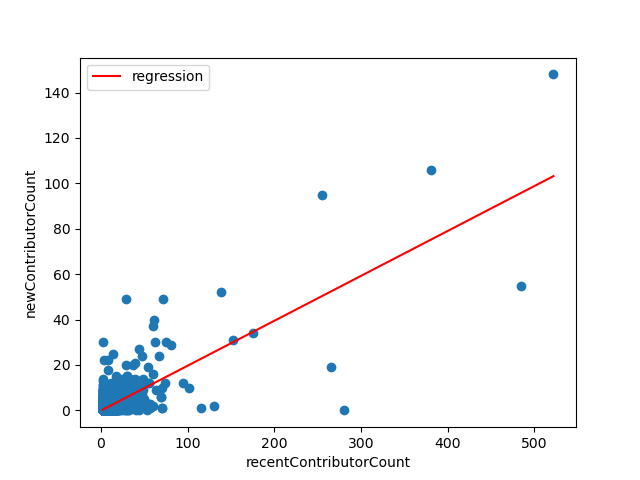
\includegraphics[width=\textwidth]{experiment/data_analysis/recentContributorCountRegression_linearScale.png}
        \caption{Échelle linéaire}
    \end{subfigure}%
    \begin{subfigure}[t]{0.5\textwidth}
        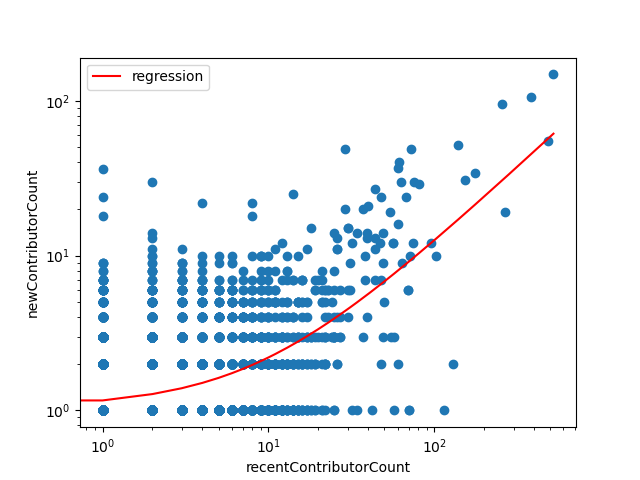
\includegraphics[width=\textwidth]{experiment/data_analysis/recentContributorCountRegression_logScale.png}
        \caption{Échelle logarithmique}
    \end{subfigure}

    $\mathit{newContributorCount} = \mathit{recentContributorCount} * 0.11540180 + 1.04427117$\\($r^2 = 0.28318792$)
    \caption{Nombre de nouveaux contributeurs en fonction du nombre de contributeurs récents uniques}
    \label{fig:contributorCount}
\end{figure}

\begin{figure}[ht]
    \centering
    \begin{subfigure}[t]{0.5\textwidth}
        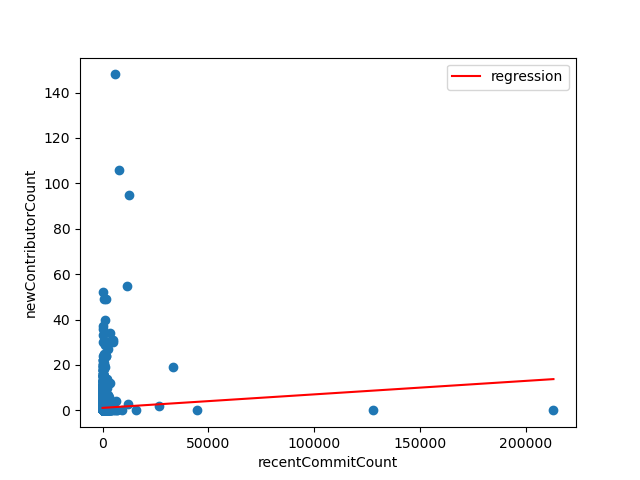
\includegraphics[width=\textwidth]{experiment/data_analysis/recentCommitCountRegression_linearScale.png}
        \caption{Échelle linéaire}
    \end{subfigure}%
    \begin{subfigure}[t]{0.5\textwidth}
        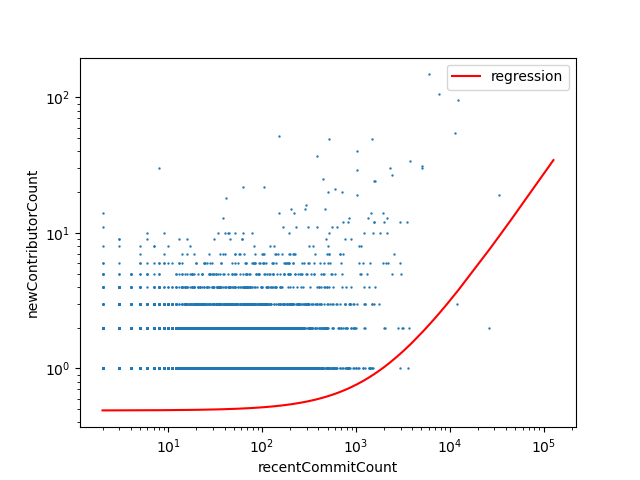
\includegraphics[width=\textwidth]{experiment/data_analysis/recentCommitCountRegression_logScale.png}
        \caption{Échelle logarithmique}
    \end{subfigure}

    $\mathit{newContributorCount} = \mathit{recentCommitCount} \times 0.00026672041 + 0.48979364$\\($r^2 = 0.12749825$)
    \caption{Nombre de nouveaux contributeurs en fonction du nombre de commits récents}
    \label{fig:commitCount}
\end{figure}

\pagelayout{margin}


\addpart{Conclusion}

\chapter{Conclusion}


% Number chapters with letters from now on
\appendix

\addpart{Annexes}

\chapter{Code d'extraction des données}

\chapter{Code de calcule des résultats}


% End of the main document content
\backmatter

\setchapterstyle{plain}

\defbibnote{bibnote}{Références utilisées, présentées par ordre de première citation.

    Les références précédées d'un astérisque désignent des études répertoriées dans des méta-analyses.

    \par\bigskip
}
\printbibliography[heading=bibintoc, prenote=bibnote]

\printindex

\printglossary



\end{document}
